This chapter discusses three main sets of simulation results. First, we
compare the key neutronics results between Serpent and Moltres for a static
model of the \gls{MSFR}, i.e. no salt flow, to assess the accuracy of the
six-group neutron diffusion model in Moltres on a fast-spectrum reactor. This
exercise also serves as a checking exercise for the group constant data
generated for Moltres from Serpent. Second, we present steady-state results
from Moltres with salt flow and verify it against published results, namely
from the Polimi/TUDelft and OpenFOAM models developed by Fiorina et al.
\cite{fiorina_modelling_2014} and Aufiero et al.
\cite{aufiero_development_2014}, respectively. Lastly, we present and compare
transient simulation results from Moltres with the aforementioned models.
Transient accident scenarios include an unprotected reactivity insertion, an
unprotected loss of flow, an unprotected loss of heat sink, a chilled inlet,
and a pump overspeed scenario.

\section{Static Model}

We calculated estimates of $k_{\text{eff}}$ values in Serpent and Moltres for
the \gls{MSFR} model with static salt (no flow), and uniform temperature
distributions. Moltres solves the six-group neutron diffusion equations as a
steady-state eigenvalue problem to find the $k_{\text{eff}}$ as it does not
currently have the capability to calculate the adjoint flux. Table
\ref{table:keff} shows the $k_{\text{eff}}$ values from Serpent and Moltres at
973 K and the corresponding salt density, while Table \ref{table:keff} shows
the $k_{\text{eff}}$ values for other temperatures at 100 K intervals. We
observe small discrepancies on the order of 100 pcm between the two codes
which we attribute to two main factors: the accuracy of the neutron diffusion
model, and the omission of the blanket tank structural material. The neutron
diffusion model is not as accurate as the other S$_{\text{N}}$ or
SP$_{\text{N}}$ deterministic methods nor the Monte Carlo approach in Serpent.
Regarding the omission of the blanket tank material, we replaced the
2 cm-thick structural material with blanket salt. This replacement may be
partly responsible for the higher $k_{\text{eff}}$ value calculated by Moltres
as the macroscopic fission cross sections of the blanket salt are non-zero for
the higher neutron energy groups. Nevertheless, the discrepancy is smaller
than the 228.5 pcm and 256.7 pcm discrepancies reported by Cervi et al.
\cite{cervi_development_2019} for their six-group $SP_3$ and neutron
diffusion methods, respectively, in OpenFOAM. The neutron diffusion model in
OpenFOAM is the same approach Aufiero et al. \cite{aufiero_development_2014}
used for their transient analysis of the \gls{MSFR}, albeit with one neutron
energy group.

\begin{table}[htb!]
    \small
	\centering
	\caption{$k_{\text{eff}}$ values from Serpent and Moltres at 973 K.}
	\begin{tabular}{l S c}
		\toprule
		{Code} & {$k_{\text{eff}}$} & {Difference wrt Serpent [pcm]}\\
		\midrule
		{Serpent} & 1.00662 \pm 0.00005 & {-}\\
		{Moltres with \glspl{DNP}} & 1.0079488 \pm 0.0000010 & 133\\
		{Moltres without \glspl{DNP}} & 1.0049369 \pm 0.0000010 & {-}\\
		\bottomrule
	\end{tabular}
	\label{table:keff}
\end{table}
%
\begin{table}[htb!]
    \small
	\centering
	\caption{$k_{\text{eff}}$ values from Serpent and Moltres at various
	temperatures from 800 K to 1400 K.}
	\begin{tabular}{S S S S}
		\toprule
		{Temperature [K]} & {$k_{\text{eff}}$ $\pm$ 1-$\sigma$ uncertainty
		(Serpent)} & {$k_{\text{eff}}$ (Moltres)} & {Difference wrt Serpent
		[pcm]}
		\\
		\midrule
		800  & 1.01996 \pm 0.00005 & 1.02117 & 121 \\
		900  & 1.01172 \pm 0.00005 & 1.01322 & 150 \\
		1000 & 1.00428 \pm 0.00005 & 1.00544 & 116 \\
		1100 & 0.99735 \pm 0.00005 & 0.99859 & 124 \\
		1200 & 0.99006 \pm 0.00005 & 0.99119 & 113 \\
		1300 & 0.98356 \pm 0.00005 & 0.98439 &  83 \\
		1400 & 0.97702 \pm 0.00005 & 0.97820 & 118 \\
		\bottomrule
	\end{tabular}
	\label{table:ktemp}
\end{table}

The absolute value of $k_{\text{eff}}$ largely impacts the steady-state
temperature of the reactor. We may adjust $k_{\text{eff}}$ by controlling
fissile inventory to raise or lower the operating temperatures and meet the
design specifications for inlet and outlet temperatures. For transient
analysis, the $\beta_{\text{eff}}$ and reactivity coefficients are arguably
more important as they dictate the duration and magnitude of the reactor
response to a transient initiator. The $\beta_{\text{eff}}$ values at 973 K,
shown in Table \ref{table:betaeff}, are in excellent agreement with a 2.89
pcm discrepancy.

\begin{table}[htb!]
	\centering
	\caption{$\beta_{\text{eff}}$ values from Serpent and Moltres at 973 K.}
	\begin{tabular}{l S S}
		\toprule
		{Code} & {$\beta_{\text{eff}}$ [pcm]} & {Difference wrt Serpent [pcm]}
		\\
		\midrule
		{Serpent} & 304.08 \pm .81 & {-}\\
		{Moltres} & 301.19 \pm .20 & 2.89\\
		\bottomrule
	\end{tabular}
	\label{table:betaeff}
\end{table}
%
\begin{figure}[htb!]
    \centering
    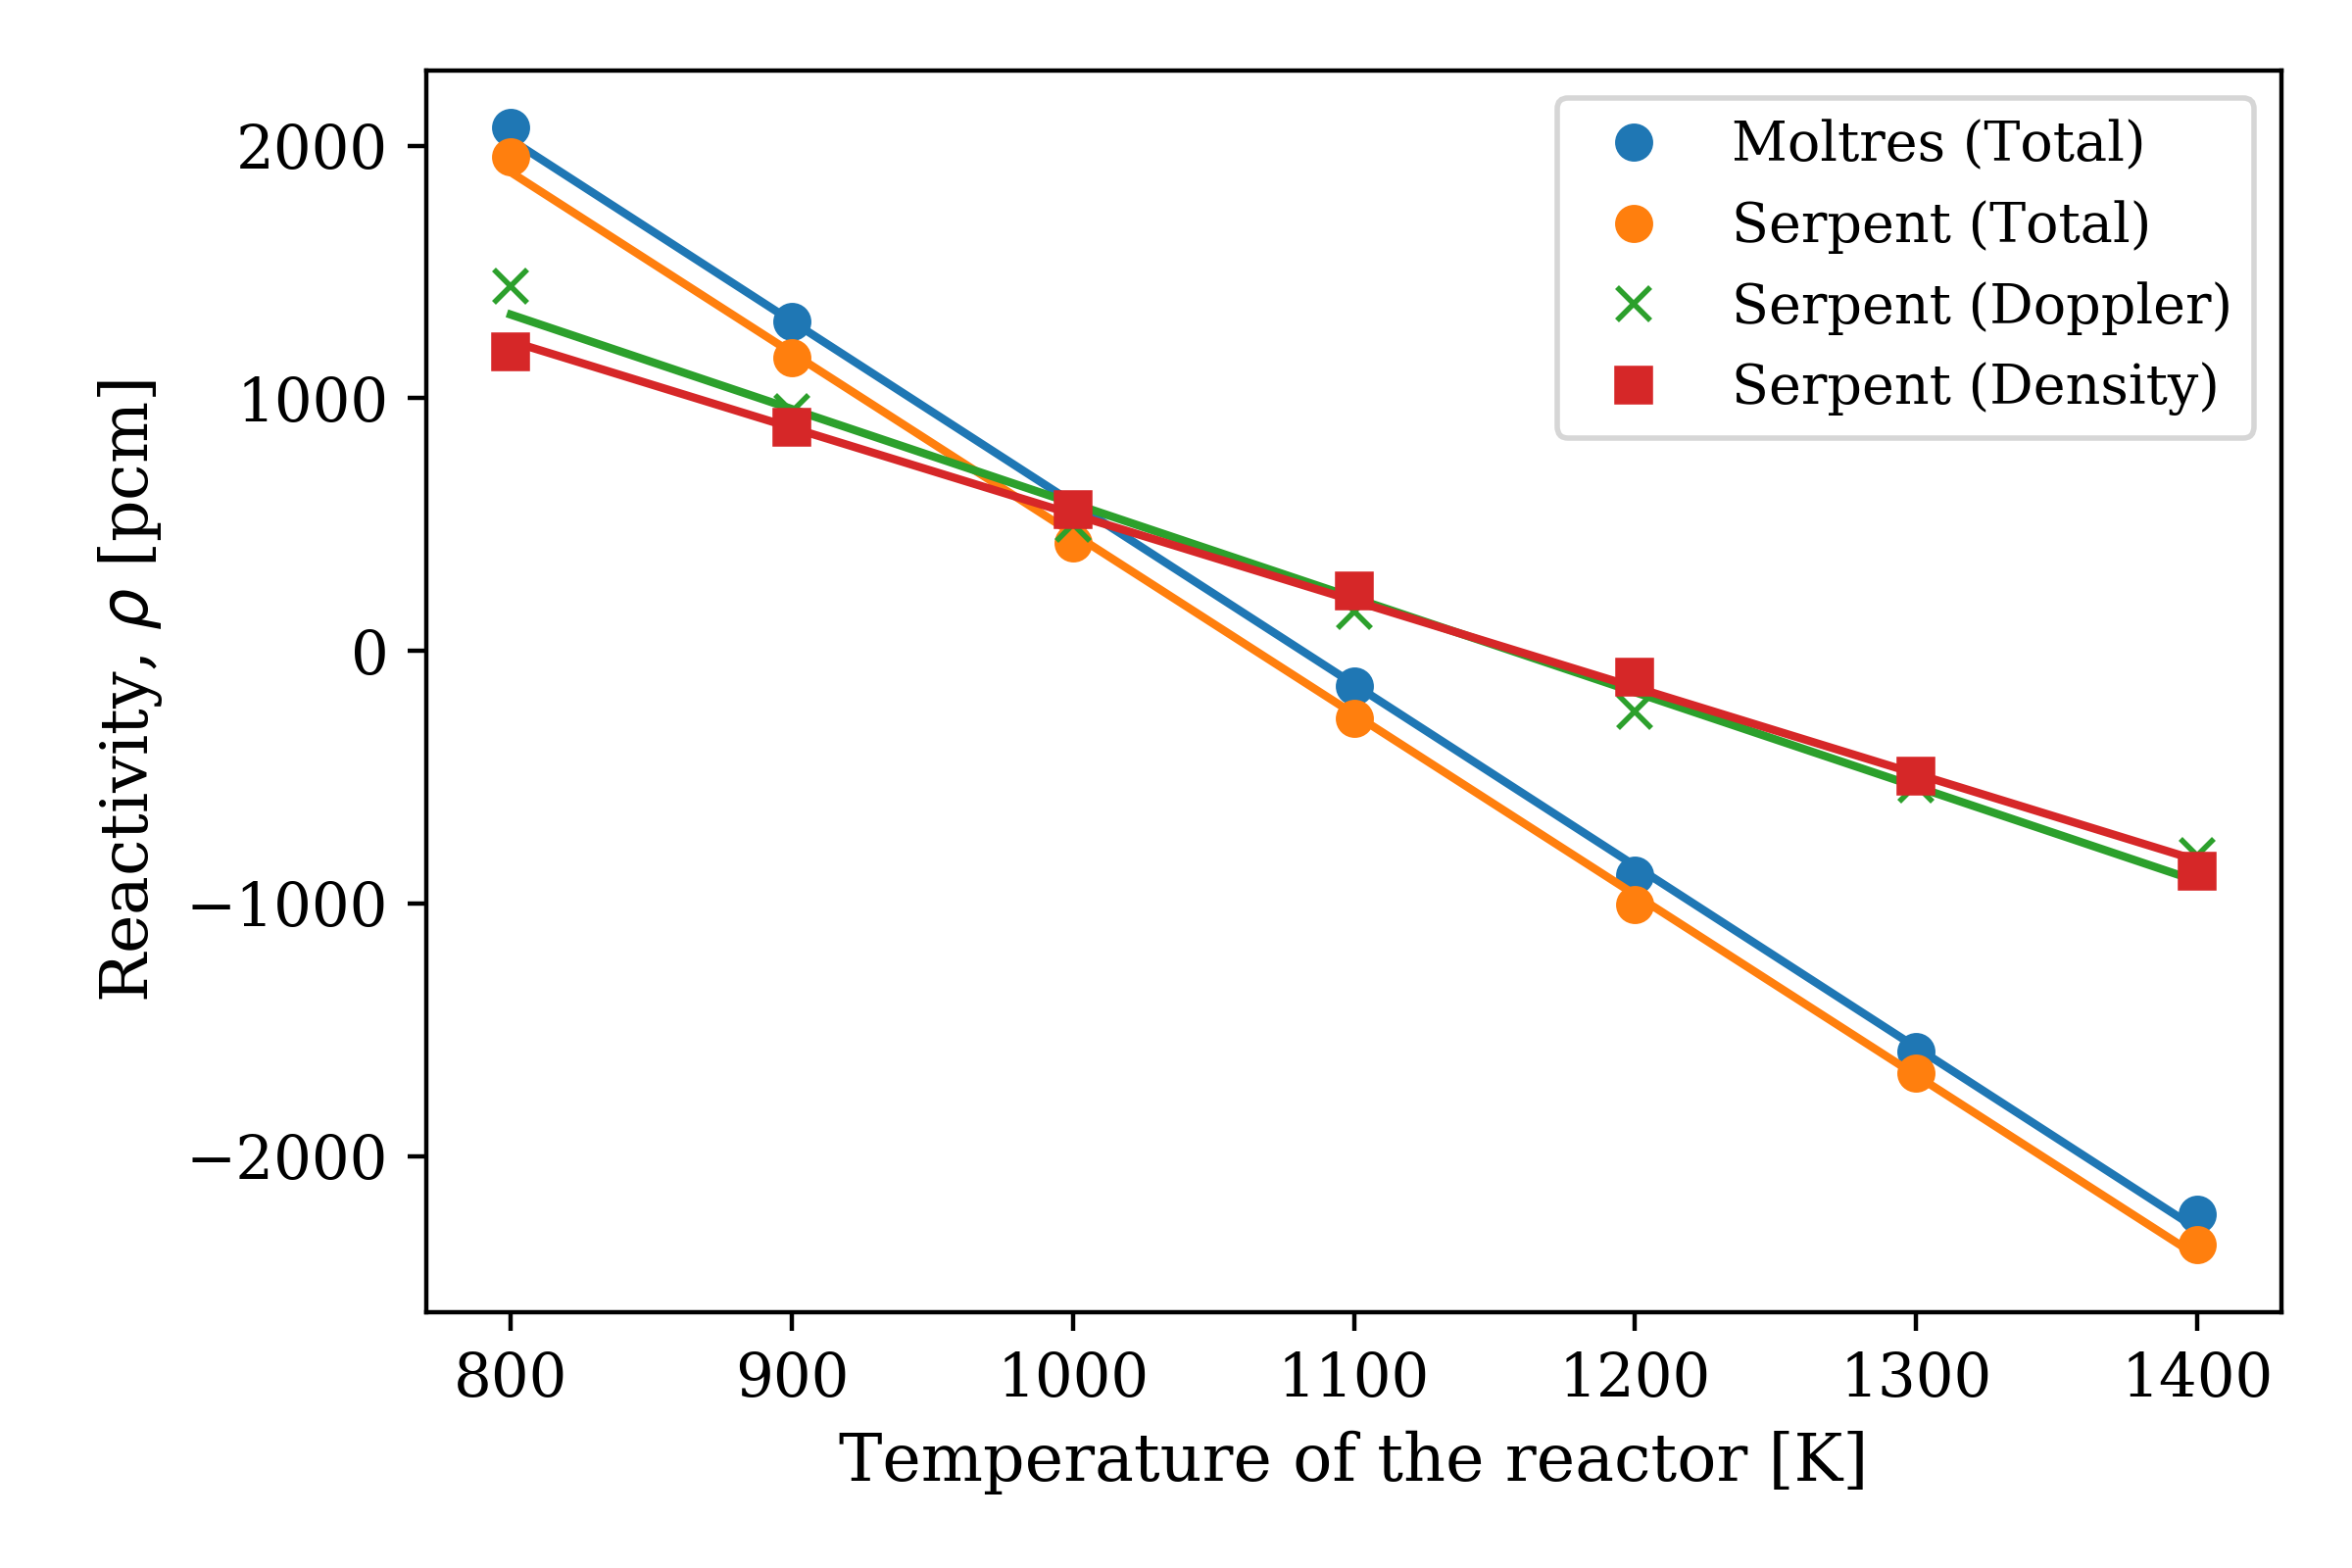
\includegraphics[width=.8\textwidth]{reactivity}
    \caption{Reactivity values from Serpent and Moltres. The Doppler
    reactivity values were calculated at a fixed density of 4.1249 g
    cm$^{-3}$. The density reactivity values were calculated at a fixed
    temperature of 973 K.}
    \label{fig:reactivity}
\end{figure}
%
\begin{table}[htb!]
	\centering
	\caption{Doppler, density, and total temperature coefficients
	for the temperature range of 800 K to 1400 K.}
	\begin{tabular}{l S S S S}
		\toprule
		{Code} & {$\alpha_D$ (log) [pcm]} & {$\alpha_D$ (linear) [pcm
		K$^{-1}$]} & {$\alpha_\rho$ [pcm K$^{-1}$]} & {$\alpha_T$ [pcm
		K$^{-1}$]} \\
		\midrule
		{Serpent} & -4034 \pm 14 & 3.737 \pm 0.013 & 3.424 \pm 0.013 & 7.165
		\pm 0.013 \\
		{Moltres} & {-} & {-} & {-} & 7.184\\
		\bottomrule
	\end{tabular}
	\label{table:alpha}
\end{table}

The temperature reactivity feedback arises mainly from Doppler broadening of
resonance absorption peaks and temperature-induced density changes. Although
Doppler coefficients typically show logarithmic dependence to temperature, we
report them, along with the other coefficients, as linear gradient
values of the reactivity given the relatively linear trend within the relevant
temperature range (Figure \ref{fig:reactivity}). Table \ref{table:alpha} shows
the temperature coefficients as described prior. The total temperature
coefficients from Serpent and Moltres show excellent agreement with a
discrepancy of 0.019 pcm K$^{-1}$.

Moltres also reproduced the six-group neutron spectrum very well from the
Serpent group constants. Figure \ref{fig:ntspec} compares the energy spectra
from Serpent and Moltres in the central fuel salt region. The six-group
neutron spectra overlap exactly over each other. More generally, the plot
shows the distinctive fast spectrum observed in the \gls{MSFR} with dips in
the spectrum corresponding to elastic scattering resonances from lithium and
fluorine. From this plot, we observe that the discrepancies in
$k_{\text{eff}}$ arise mainly from discretizing neutron energy into groups
rather than the neutron diffusion model itself. We could obtain a more
accurate representation of the neutronics in the \gls{MSFR} by using more
neutron energy groups but this would adversely impact simulation times in the
subsequent multiphysics finite element analyses.

\begin{figure}[htb!]
    \centering
    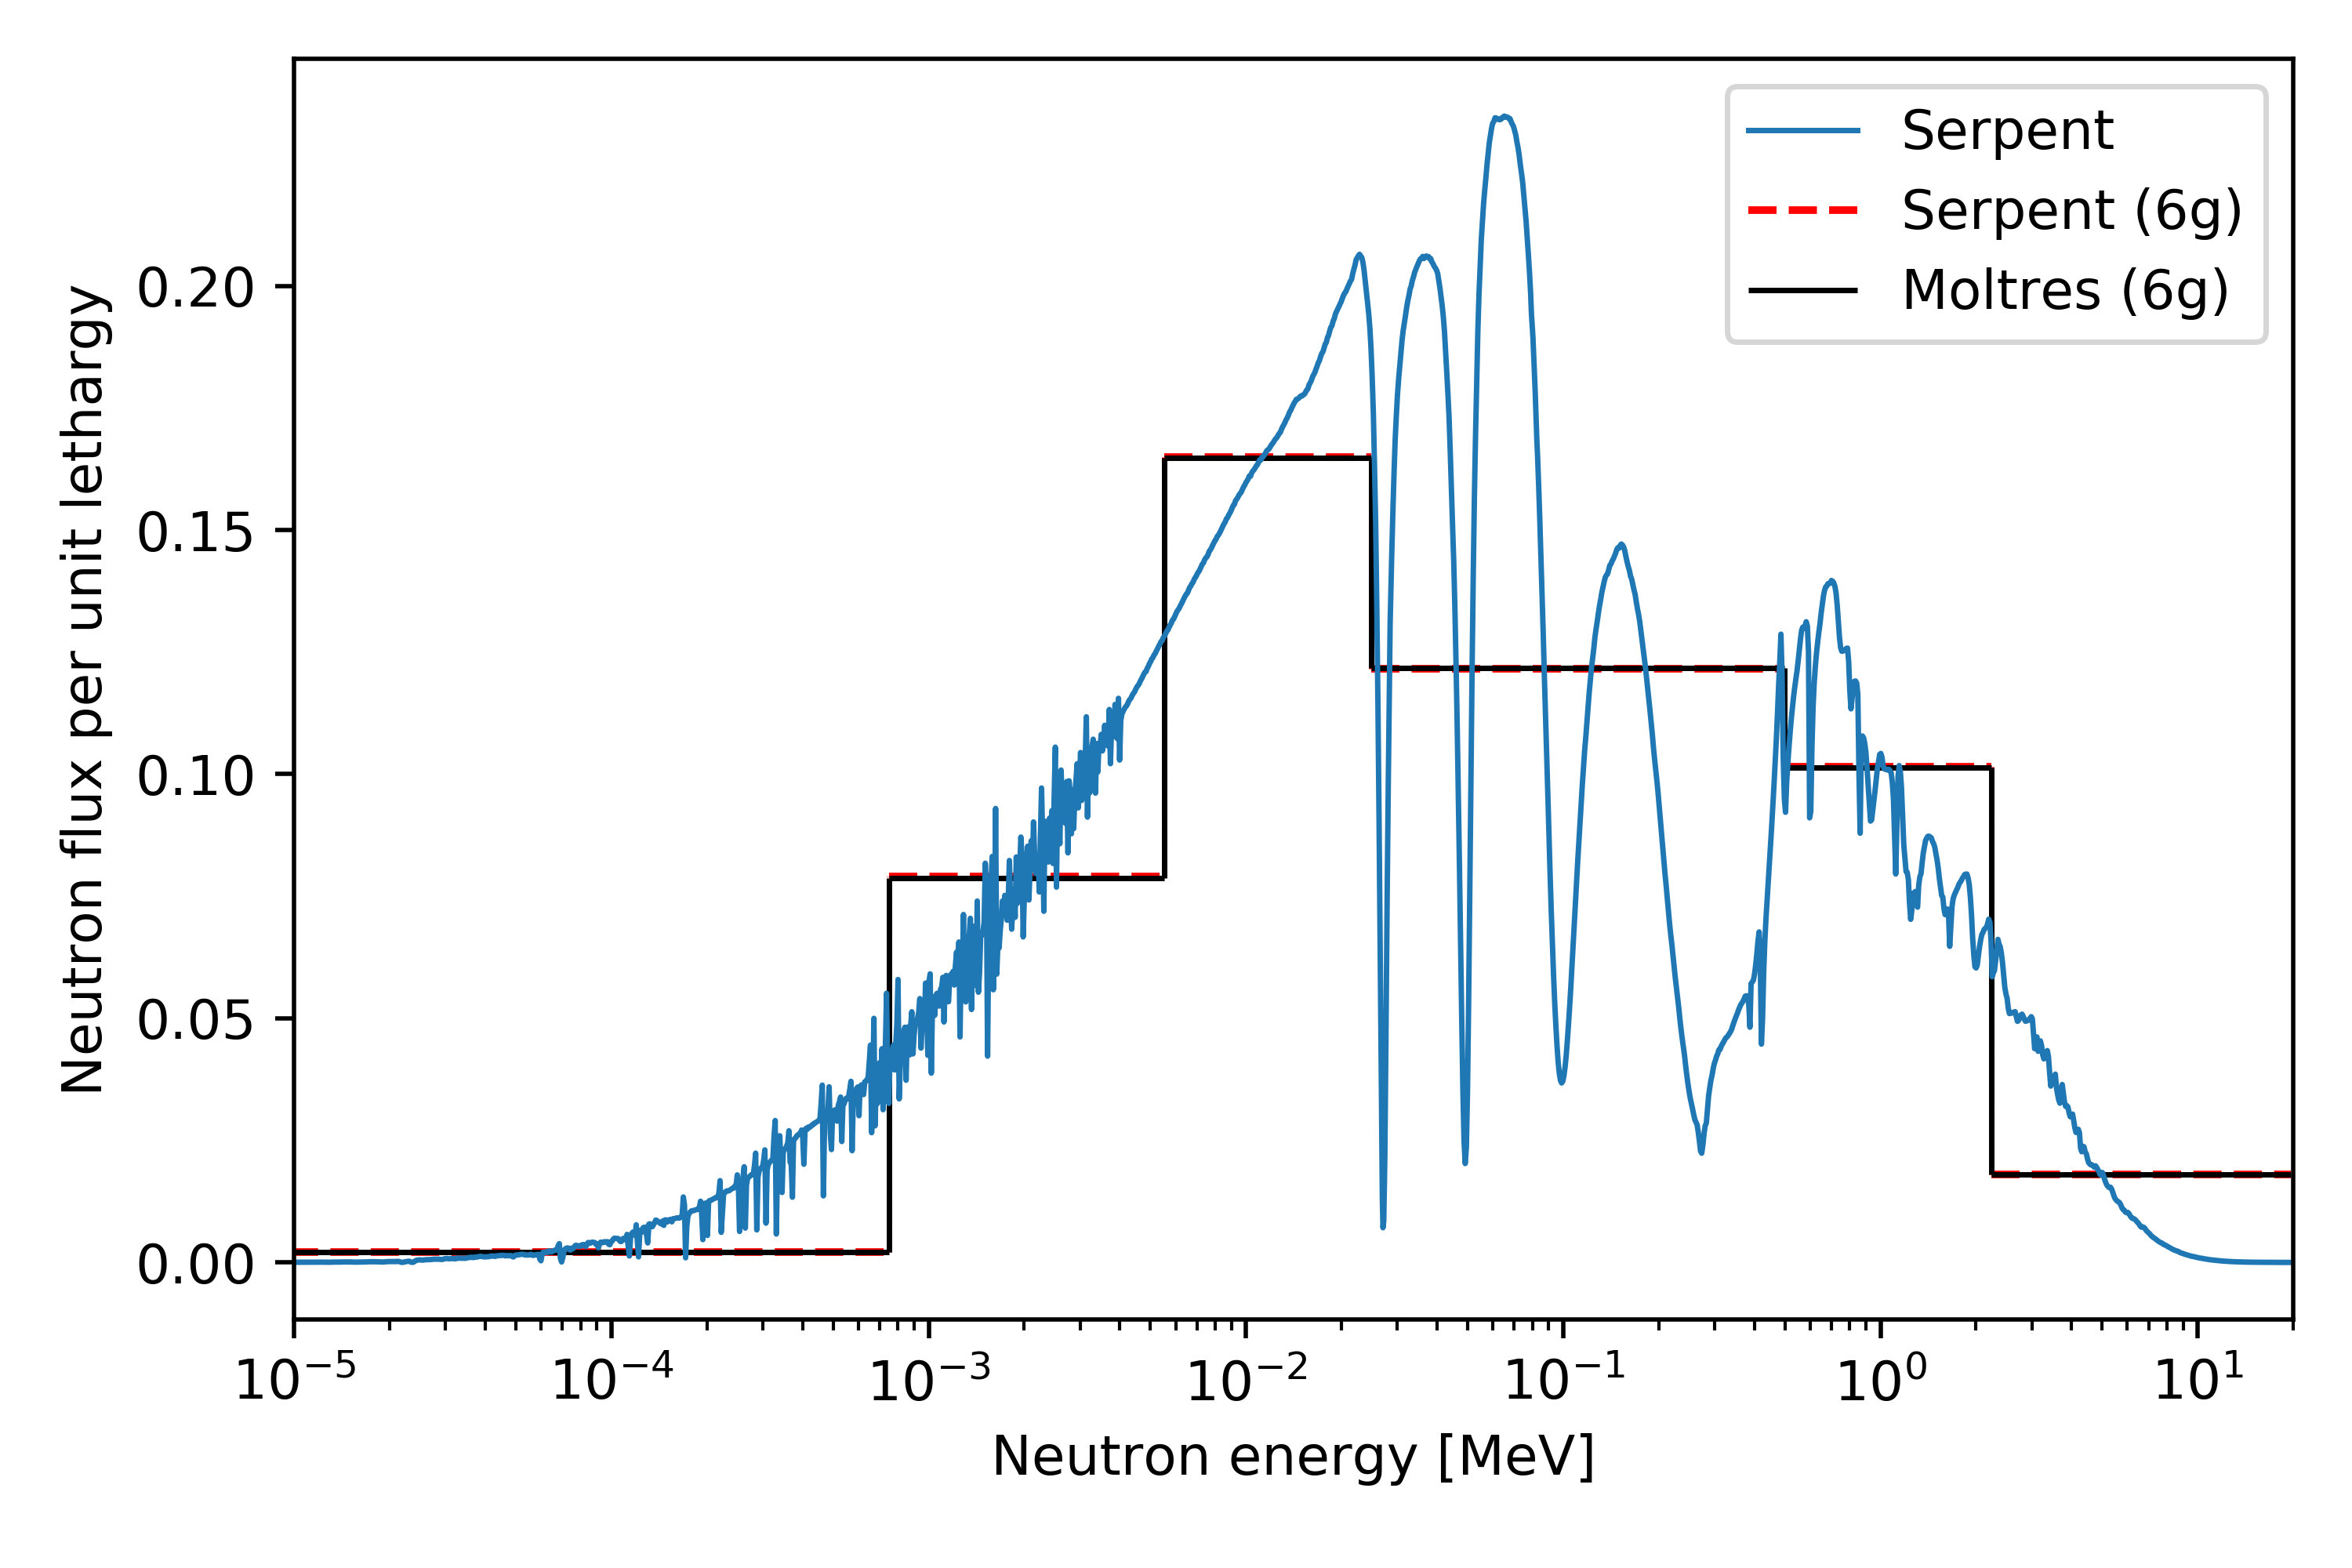
\includegraphics[width=.8\textwidth]{nt-spec}
    \caption{Reactivity values from Serpent and Moltres. The Doppler
    reactivity values were calculated at a fixed density of 4.1249 g
    cm$^{-3}$. The density reactivity values were calculated at a fixed
    temperature of 973 K.}
    \label{fig:ntspec}
\end{figure}

In summary, Moltres can replicate most of the relevant neutronics parameters
accurately with the group constant data from Serpent. While the
$k_{\text{eff}}$ values have discrepancies on the order of 100 pcm, they are
relatively small compared to results from other codes. Furthermore, the
$\beta_{\text{eff}}$ and temperature coefficients, which are important
parameters for modeling transient reactor behavior, are in excellent
agreement.

\section{Steady-State Results}

With the verification of Moltres' neutronics modeling capabilities in the
context of the \gls{MSFR}, we now move on to the multiphysics simulation
results. This section covers the steady-state multiphysics results from
Moltres.

The procedure for obtaining the steady-state results involved several steps
due to the highly coupled \glspl{PDE}. First, we ran a preliminary transient
simulation of fluid flow in the gls\MSFR} core, starting from zero inlet
velocity and gradually ramping it up to match the nominal flow rate (4.5 m$^3$
s$^{-1}$); otherwise Moltres had difficulty converging to the desired fully
developed flow profile. We imposed a parabolic flow profile at the inlet.
Next, we imported these fully developed flow values as initial values for
velocity in the actual transient simulation modeling the full coupled
neutronics and thermal-hydraulics. The initial values for the temperature and
neutron group flux distributions are 953 K and $1 \times 10^{14}$ cm$^{-2}$
s$^{-1}$ uniformly throughout the geometry. Finally, we assume that steady
state is reached when the volume integral values of every variable remain
constant (up to 6 sig. fig.) for at least four seconds in the simulation; this
time period corresponds to the nominal circulation time of the \gls{MSFR}.

For a direct comparison with the steady-state results from the Polimi/TUDelft
models, the bulk of our steady-state results do not have decay heat modeling.
Instead, we separately discuss the minor differences borne from decay heat
modeling in the last subsection.

\subsection{Thermal-Hydraulics}

Figure \ref{fig:flow-temp} shows the temperature and velocity fields
of the fuel salt in the core at steady state from Moltres and the
Polimi/TUDelft models. The results from Moltres show good qualitative
agreement with the Polimi/TUDelft models; we observe similar flow and hotspot
features in all three models. There is a large recirculation region near the
blanket tank walls arising from turbulent flow. Inertial forces dominate over
viscous forces to form this large eddy. The figure also shows two relatively
stagnant regions along the central axis at the top and bottom of the core.
Temperature hotspots form in these regions of recirculation as convection is
the dominant heat transfer mechanism. The maximum temperature from Moltres,
1279 K near the bottom of the recirculation zone, is closer to the maximum
temperature in the Polimi model ($\approx$ 1300 K) than the TUDelft model
($\approx$ 1200K). The minimum temperature is 922 K at the inlet. Figure
\ref{fig:flow} provides an alternate view of the flow profile through flow
streamlines superimposed on the velocity magnitude distribution. The fastest
salt flow occurs at the inlet, outlet, and at core half-height approximately
0.40 m away from the central axis.

\begin{figure}[htb!]
    \centering
    \begin{subfigure}[t]{.37\textwidth}
        \centering
        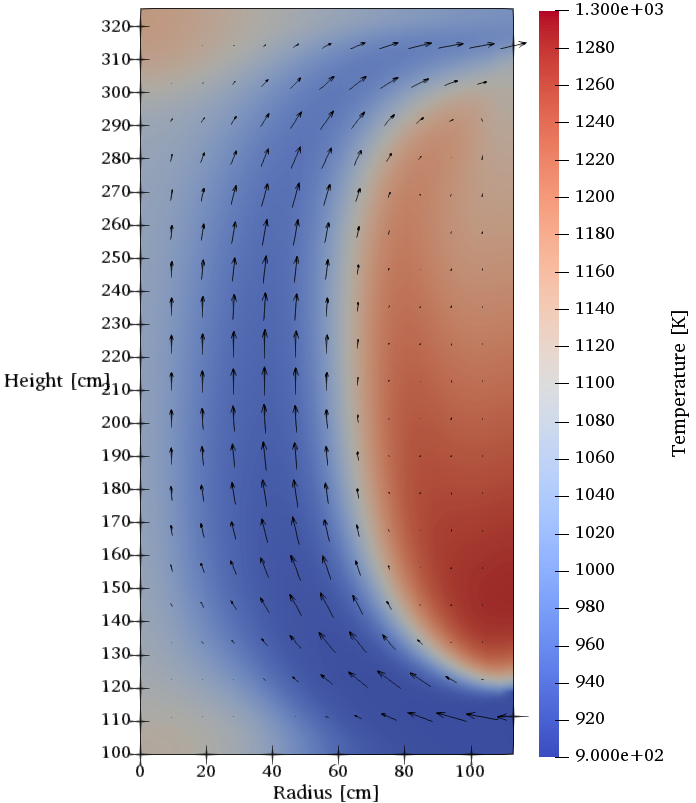
\includegraphics[width=\textwidth]{flow-temp}
    \end{subfigure}
    \hfill
    \begin{subfigure}[t]{.625\textwidth}
        \centering
        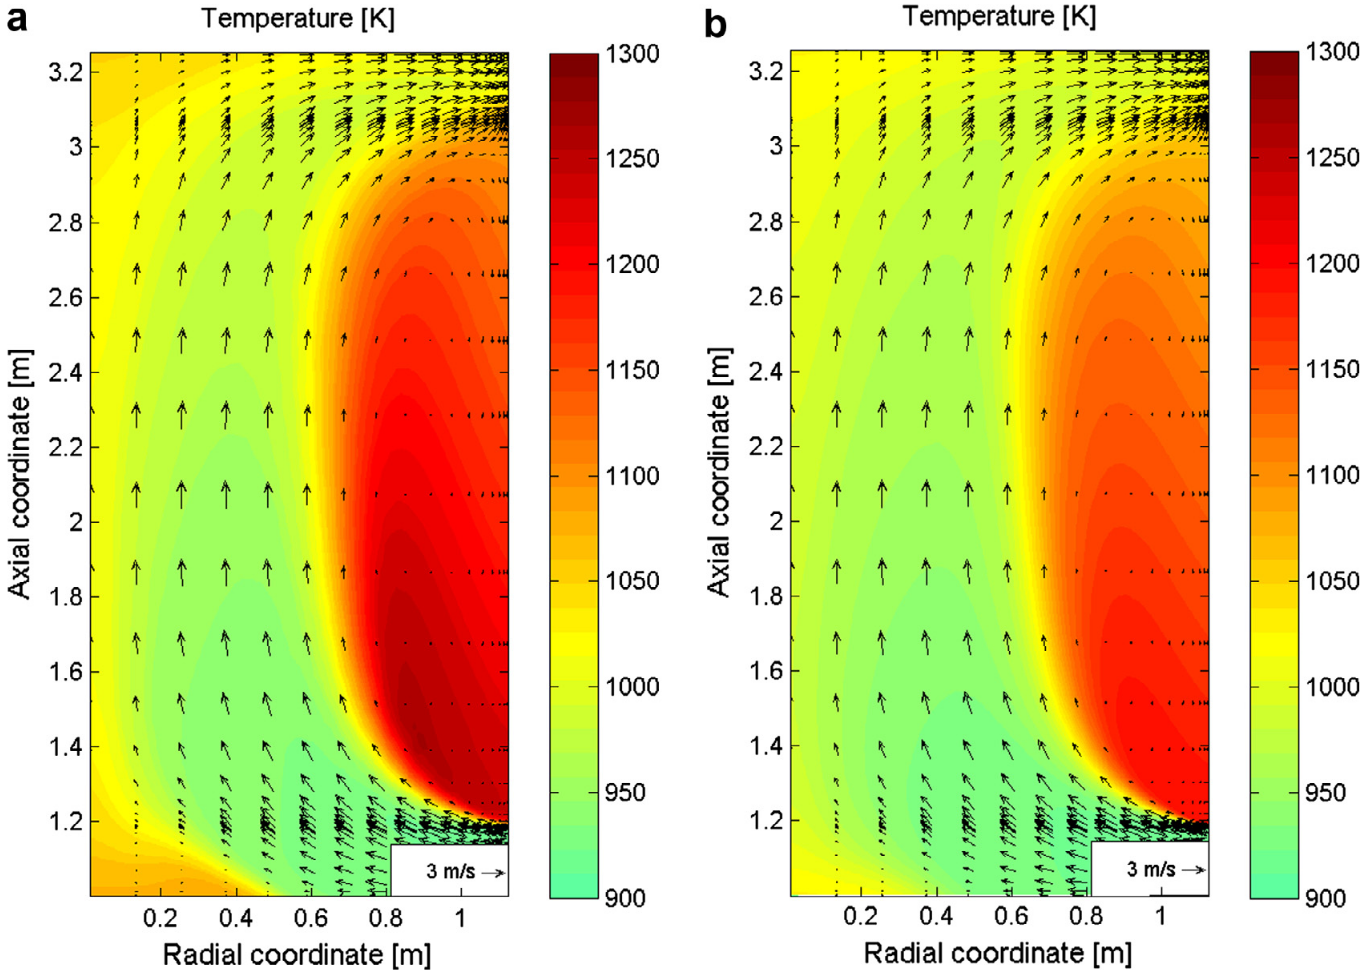
\includegraphics[width=\textwidth]{flow-temp-fiorina}
    \end{subfigure}
    \caption{Temperature and velocity fields in the core from Moltres
    (left), Polimi (center), and TUDelft (right) models.}
    \label{fig:flow-temp}
\end{figure}

\begin{figure}[htb!]
    \centering
    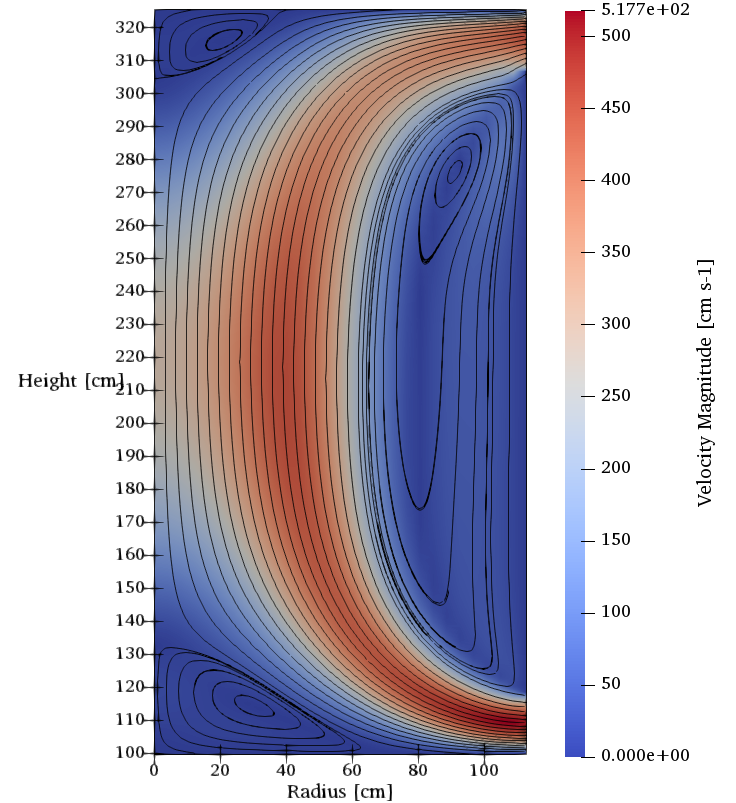
\includegraphics[width=.6\textwidth]{flow}
    \caption{Fuel salt flow streamlines and velocity magnitude in the core.}
    \label{fig:flow}
\end{figure}

While the temperatures at the hotspots are well below the melting point of the
Ni-alloy structure (1500 K), they may cause undue thermal stress on the
blanket tank structure and induce relatively faster salt corrosion rates. A
sudden, large reactivity insertion could push fuel salt temperatures above the
melting point of the Ni-alloy and cause irreversible damage. Furthermore,
the reservoir of hot fuel salt may cause unpredictable behavior during
transient scenarios when the flow profile undergoes a drastic change.
Thus, Rouch et al. \cite{rouch_preliminary_2014} developed an improved
hourglass-shaped design to optimize flow distribution and prevent these
recirculation zones and hotspots from forming. A study of this new design
using Moltres is a potential subject for future work when a proper turbulence
model is in place.

\subsection{Neutronics}



\subsection{Decay Heat}

A decay heat model effectively redistributes a fraction of the heat source
from the center of the core to the entire loop. Thus, we expect to observe
a slight flattening of the temperature distribution across the entire primary
loop.

\section{Transient Results}

As noted by Fiorina et al. \cite{fiorina_modelling_2014}, explicit decay heat
modeling has a negligible effect on reactivity-, pump-, and enchanced
cooling-driven transients. The Polimi model presented results with the decay
heat model for the loss of heat sink transient scenario only. For a fair
comparison, we also 

\subsection{Unprotected Reactivity Insertion}

\subsection{Unprotected Loss of Flow}

\subsection{Unprotected Loss of Heat Sink}

\subsection{Chilled Inlet}

\subsection{Pump Overspeed}
